% Options for packages loaded elsewhere
\PassOptionsToPackage{unicode}{hyperref}
\PassOptionsToPackage{hyphens}{url}
\PassOptionsToPackage{dvipsnames,svgnames,x11names}{xcolor}
%
\documentclass[
  super,
  preprint,
  3p]{elsarticle}

\usepackage{amsmath,amssymb}
\usepackage{iftex}
\ifPDFTeX
  \usepackage[T1]{fontenc}
  \usepackage[utf8]{inputenc}
  \usepackage{textcomp} % provide euro and other symbols
\else % if luatex or xetex
  \usepackage{unicode-math}
  \defaultfontfeatures{Scale=MatchLowercase}
  \defaultfontfeatures[\rmfamily]{Ligatures=TeX,Scale=1}
\fi
\usepackage{lmodern}
\ifPDFTeX\else  
    % xetex/luatex font selection
\fi
% Use upquote if available, for straight quotes in verbatim environments
\IfFileExists{upquote.sty}{\usepackage{upquote}}{}
\IfFileExists{microtype.sty}{% use microtype if available
  \usepackage[]{microtype}
  \UseMicrotypeSet[protrusion]{basicmath} % disable protrusion for tt fonts
}{}
\makeatletter
\@ifundefined{KOMAClassName}{% if non-KOMA class
  \IfFileExists{parskip.sty}{%
    \usepackage{parskip}
  }{% else
    \setlength{\parindent}{0pt}
    \setlength{\parskip}{6pt plus 2pt minus 1pt}}
}{% if KOMA class
  \KOMAoptions{parskip=half}}
\makeatother
\usepackage{xcolor}
\setlength{\emergencystretch}{3em} % prevent overfull lines
\setcounter{secnumdepth}{5}
% Make \paragraph and \subparagraph free-standing
\ifx\paragraph\undefined\else
  \let\oldparagraph\paragraph
  \renewcommand{\paragraph}[1]{\oldparagraph{#1}\mbox{}}
\fi
\ifx\subparagraph\undefined\else
  \let\oldsubparagraph\subparagraph
  \renewcommand{\subparagraph}[1]{\oldsubparagraph{#1}\mbox{}}
\fi

\usepackage{color}
\usepackage{fancyvrb}
\newcommand{\VerbBar}{|}
\newcommand{\VERB}{\Verb[commandchars=\\\{\}]}
\DefineVerbatimEnvironment{Highlighting}{Verbatim}{commandchars=\\\{\}}
% Add ',fontsize=\small' for more characters per line
\usepackage{framed}
\definecolor{shadecolor}{RGB}{241,243,245}
\newenvironment{Shaded}{\begin{snugshade}}{\end{snugshade}}
\newcommand{\AlertTok}[1]{\textcolor[rgb]{0.68,0.00,0.00}{#1}}
\newcommand{\AnnotationTok}[1]{\textcolor[rgb]{0.37,0.37,0.37}{#1}}
\newcommand{\AttributeTok}[1]{\textcolor[rgb]{0.40,0.45,0.13}{#1}}
\newcommand{\BaseNTok}[1]{\textcolor[rgb]{0.68,0.00,0.00}{#1}}
\newcommand{\BuiltInTok}[1]{\textcolor[rgb]{0.00,0.23,0.31}{#1}}
\newcommand{\CharTok}[1]{\textcolor[rgb]{0.13,0.47,0.30}{#1}}
\newcommand{\CommentTok}[1]{\textcolor[rgb]{0.37,0.37,0.37}{#1}}
\newcommand{\CommentVarTok}[1]{\textcolor[rgb]{0.37,0.37,0.37}{\textit{#1}}}
\newcommand{\ConstantTok}[1]{\textcolor[rgb]{0.56,0.35,0.01}{#1}}
\newcommand{\ControlFlowTok}[1]{\textcolor[rgb]{0.00,0.23,0.31}{#1}}
\newcommand{\DataTypeTok}[1]{\textcolor[rgb]{0.68,0.00,0.00}{#1}}
\newcommand{\DecValTok}[1]{\textcolor[rgb]{0.68,0.00,0.00}{#1}}
\newcommand{\DocumentationTok}[1]{\textcolor[rgb]{0.37,0.37,0.37}{\textit{#1}}}
\newcommand{\ErrorTok}[1]{\textcolor[rgb]{0.68,0.00,0.00}{#1}}
\newcommand{\ExtensionTok}[1]{\textcolor[rgb]{0.00,0.23,0.31}{#1}}
\newcommand{\FloatTok}[1]{\textcolor[rgb]{0.68,0.00,0.00}{#1}}
\newcommand{\FunctionTok}[1]{\textcolor[rgb]{0.28,0.35,0.67}{#1}}
\newcommand{\ImportTok}[1]{\textcolor[rgb]{0.00,0.46,0.62}{#1}}
\newcommand{\InformationTok}[1]{\textcolor[rgb]{0.37,0.37,0.37}{#1}}
\newcommand{\KeywordTok}[1]{\textcolor[rgb]{0.00,0.23,0.31}{#1}}
\newcommand{\NormalTok}[1]{\textcolor[rgb]{0.00,0.23,0.31}{#1}}
\newcommand{\OperatorTok}[1]{\textcolor[rgb]{0.37,0.37,0.37}{#1}}
\newcommand{\OtherTok}[1]{\textcolor[rgb]{0.00,0.23,0.31}{#1}}
\newcommand{\PreprocessorTok}[1]{\textcolor[rgb]{0.68,0.00,0.00}{#1}}
\newcommand{\RegionMarkerTok}[1]{\textcolor[rgb]{0.00,0.23,0.31}{#1}}
\newcommand{\SpecialCharTok}[1]{\textcolor[rgb]{0.37,0.37,0.37}{#1}}
\newcommand{\SpecialStringTok}[1]{\textcolor[rgb]{0.13,0.47,0.30}{#1}}
\newcommand{\StringTok}[1]{\textcolor[rgb]{0.13,0.47,0.30}{#1}}
\newcommand{\VariableTok}[1]{\textcolor[rgb]{0.07,0.07,0.07}{#1}}
\newcommand{\VerbatimStringTok}[1]{\textcolor[rgb]{0.13,0.47,0.30}{#1}}
\newcommand{\WarningTok}[1]{\textcolor[rgb]{0.37,0.37,0.37}{\textit{#1}}}

\providecommand{\tightlist}{%
  \setlength{\itemsep}{0pt}\setlength{\parskip}{0pt}}\usepackage{longtable,booktabs,array}
\usepackage{calc} % for calculating minipage widths
% Correct order of tables after \paragraph or \subparagraph
\usepackage{etoolbox}
\makeatletter
\patchcmd\longtable{\par}{\if@noskipsec\mbox{}\fi\par}{}{}
\makeatother
% Allow footnotes in longtable head/foot
\IfFileExists{footnotehyper.sty}{\usepackage{footnotehyper}}{\usepackage{footnote}}
\makesavenoteenv{longtable}
\usepackage{graphicx}
\makeatletter
\def\maxwidth{\ifdim\Gin@nat@width>\linewidth\linewidth\else\Gin@nat@width\fi}
\def\maxheight{\ifdim\Gin@nat@height>\textheight\textheight\else\Gin@nat@height\fi}
\makeatother
% Scale images if necessary, so that they will not overflow the page
% margins by default, and it is still possible to overwrite the defaults
% using explicit options in \includegraphics[width, height, ...]{}
\setkeys{Gin}{width=\maxwidth,height=\maxheight,keepaspectratio}
% Set default figure placement to htbp
\makeatletter
\def\fps@figure{htbp}
\makeatother

\makeatletter
\makeatother
\makeatletter
\makeatother
\makeatletter
\@ifpackageloaded{caption}{}{\usepackage{caption}}
\AtBeginDocument{%
\ifdefined\contentsname
  \renewcommand*\contentsname{Table of contents}
\else
  \newcommand\contentsname{Table of contents}
\fi
\ifdefined\listfigurename
  \renewcommand*\listfigurename{List of Figures}
\else
  \newcommand\listfigurename{List of Figures}
\fi
\ifdefined\listtablename
  \renewcommand*\listtablename{List of Tables}
\else
  \newcommand\listtablename{List of Tables}
\fi
\ifdefined\figurename
  \renewcommand*\figurename{Figure}
\else
  \newcommand\figurename{Figure}
\fi
\ifdefined\tablename
  \renewcommand*\tablename{Table}
\else
  \newcommand\tablename{Table}
\fi
}
\@ifpackageloaded{float}{}{\usepackage{float}}
\floatstyle{ruled}
\@ifundefined{c@chapter}{\newfloat{codelisting}{h}{lop}}{\newfloat{codelisting}{h}{lop}[chapter]}
\floatname{codelisting}{Listing}
\newcommand*\listoflistings{\listof{codelisting}{List of Listings}}
\makeatother
\makeatletter
\@ifpackageloaded{caption}{}{\usepackage{caption}}
\@ifpackageloaded{subcaption}{}{\usepackage{subcaption}}
\makeatother
\makeatletter
\@ifpackageloaded{tcolorbox}{}{\usepackage[skins,breakable]{tcolorbox}}
\makeatother
\makeatletter
\@ifundefined{shadecolor}{\definecolor{shadecolor}{rgb}{.97, .97, .97}}
\makeatother
\makeatletter
\makeatother
\makeatletter
\makeatother
\journal{Journal Name}
\ifLuaTeX
  \usepackage{selnolig}  % disable illegal ligatures
\fi
\usepackage[]{natbib}
\bibliographystyle{elsarticle-num}
\IfFileExists{bookmark.sty}{\usepackage{bookmark}}{\usepackage{hyperref}}
\IfFileExists{xurl.sty}{\usepackage{xurl}}{} % add URL line breaks if available
\urlstyle{same} % disable monospaced font for URLs
\hypersetup{
  pdftitle={Discard and bycatch monitoring program at industrial demersal fisheries in Chile: Where we are eight years from its implementation?},
  pdfauthor={Marcelo A. San Martin; EL YEI CI},
  pdfkeywords={Discard, bycatch, demersal fisheries},
  colorlinks=true,
  linkcolor={blue},
  filecolor={Maroon},
  citecolor={Blue},
  urlcolor={Blue},
  pdfcreator={LaTeX via pandoc}}

\setlength{\parindent}{6pt}
\begin{document}

\begin{frontmatter}
\title{Discard and bycatch monitoring program at industrial demersal
fisheries in Chile: Where we are eight years from its implementation?}
\author[1]{Marcelo A. San Martin%
\corref{cor1}%
\fnref{fn1}}
 \ead{marcelo.sanmartin@ifop.cl} 
\author[1]{EL YEI CI%
%
}


\affiliation[1]{organization={Instituto de Fomento Pesquero
(IFOP), Fisheries Department},addressline={Blanco
839},city={Valparaiso},postcode={Chile},postcodesep={}}
\affiliation[2]{organization={},,postcodesep={}}

\cortext[cor1]{Corresponding author}
\fntext[fn1]{This is the first author footnote.}

        
\begin{abstract}
Discard and bycatch have been a problem in world fisheries. During 2012,
modifications on the Chilean Fisheries Law, including a permanent
discard and bycatch research monitoring program (DBRMP) through
scientific observers on-board in fisheries, were established to know and
address this problem. With the aim of showing the steps and evolution of
this process, indicators of discard and bycatch at demersal industrial
fisheries between 2013 and 2020 years were assessed. Additionally, a
summary of main regulatory measures were identified. The results showed
that the involvement of fishermen was an important element to ensure the
success of DBRMP and development of discard reduction plans. One of the
biggest challenges to start the DBRMP was to achieve the engagement of
them in a participatory process. Thus, meetings were held to provide
information outreach about the law and DBRMP. After eight years from the
beginning of the DBRMP, important improvements have been observed.
Discard in trawling fisheries decreased on average 70\% respect to
initial values, while in long-line fisheries dropped 60\%. Same trend
was observed regarding bycatch of seabirds and sea lions. These results
represent a key input to understand the discard problematic and the
difficulties associated with their measurement, as well as the
understanding of the underlying causes and solutions. Among the
mandatory measures that has been implemented are; the discard ban of
target species, adjustment of the non-target species catch rate,
prohibition of bycatch, the mandatory use of bycatch mitigation measures
systems as the grid device and tori lines used to avoid sea lions and
seabirds, and the recent implementation of electronic monitoring. This
work shows a brief overview of the main advances and solutions taken by
Chilean fisheries government institutions regarding discard and bycatch,
hoping to serve as a guideline for other countries which are advocated
to address this matter.
\end{abstract}





\begin{keyword}
    Discard, bycatch \sep 
    demersal fisheries
\end{keyword}
\end{frontmatter}
    \ifdefined\Shaded\renewenvironment{Shaded}{\begin{tcolorbox}[enhanced, sharp corners, borderline west={3pt}{0pt}{shadecolor}, frame hidden, breakable, interior hidden, boxrule=0pt]}{\end{tcolorbox}}\fi

\textbf{Introduction}

Discard and bycatch have been a problem in world fisheries. Considering
the significant decreases in fish landing as of 1995 and increasing of
stocks overfished, during 2012, modifications on the Chilean Fisheries
Law with an ecosystem approach, including a permanent discard and
bycatch research monitoring program (DBRMP) through scientific observers
on-board in fisheries, were established to know and address this problem
(SanMartin2016; Roman2021). The main objectives of this monitoring
program included the determination of levels of discards in each
fishery, quantify bycatch (marine mammals, seabirds and marine turtles)
and identify the causes. Results obtained by DBRMP have been key to
implement the mandatory reduction measures to reduce the levels of
discard and bycatch at industrial demersal fisheries in Chile.

\textbf{Monitoring approach}

With the aim of showing the steps and evolution of this process,
indicators of discard and bycatch at demersal industrial fisheries
between 2013 and 2020 years were assessed. A total of ten industrial
fisheries, distributed from 28�S to 57�S, including longline and
trawling gear were considered (Figure~\ref{fig-1}).� Additionally, a
summary of main regulatory measures were identified.

\begin{figure}

{\centering 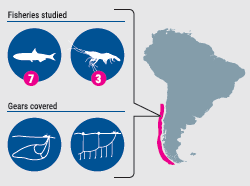
\includegraphics{fig1.png}

}

\caption{\label{fig-1}Chilean industrial demersal fisheries studied and
spatial coverage}

\end{figure}

\textbf{Results}

The results showed that the involvement of fishermen was an important
element to ensure the success of DBRMP and development of discard
reduction plans. One of the biggest challenges to start the DBRMP was to
achieve the engagement of them in a participatory process. Thus,
meetings were held to provide information outreach about the law and
DBRMP. After eight years from the beginning of the DBRMP, important
improvements have been observed. Discard in trawling fisheries showed
variations in period evaluated, but in general decreased on average 70\%
respect to initial values. The same trend was observed in long-line
fisheries, dropping around 60\% with respect to the first years (Figure
2 A). Similar trend was observed regarding bycatch of seabirds and sea
lions, nonetheless, longline fisheries have not registered bycatch of
marine mammals and bycatch of seabird has been almost absent at
crustacean fisheries (Figure 2, B y C). Four general kinds of causes of
discard were identified; regulations, operational, quality and factors
associated with commercial issues. The last cause was the most important
with factors such as catch of non-commercial species and non-commercial
size. Bycatch of sea lions and seabirds were associated with
entanglement and when the animals feeding the catch or bait.

\begin{figure}

{\centering 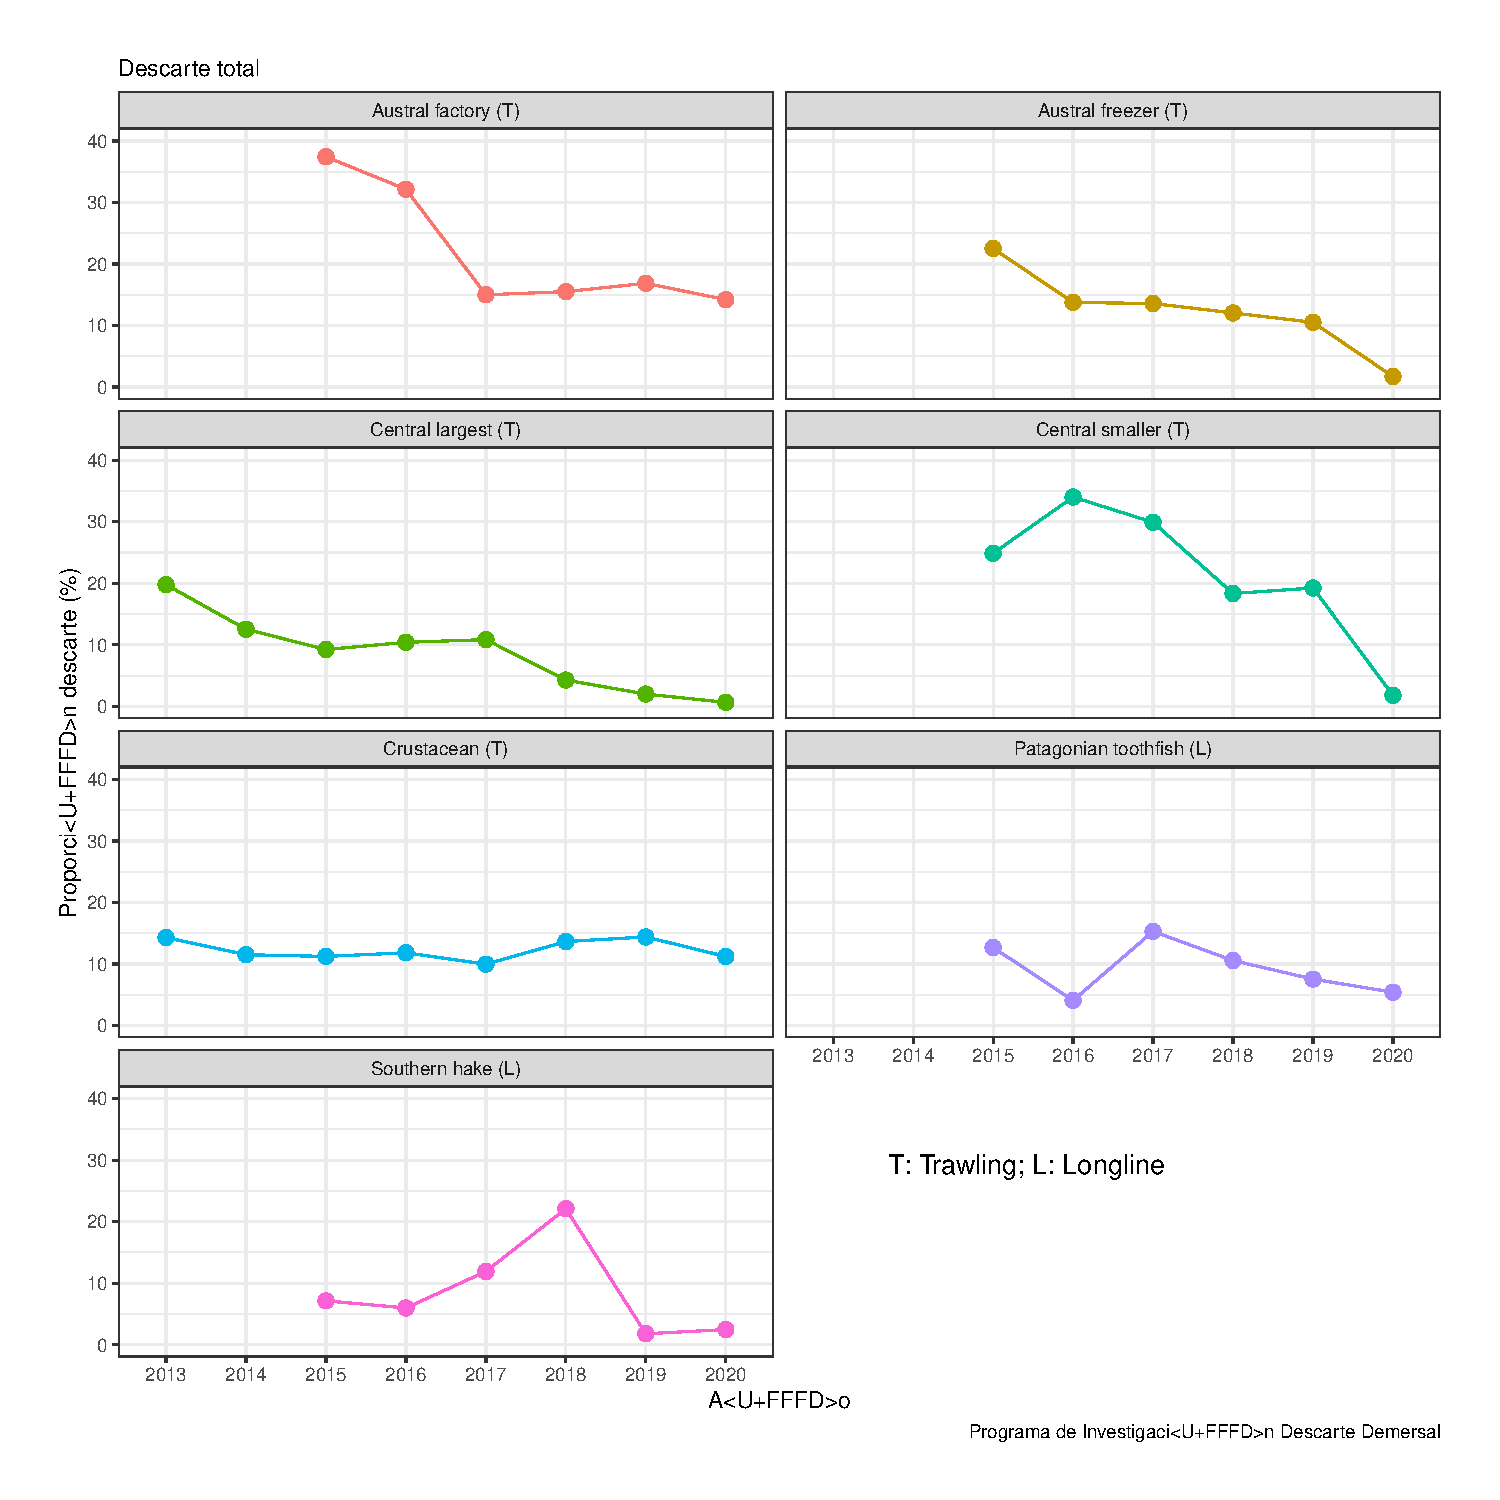
\includegraphics[width=0.4\textwidth,height=\textheight]{Tarea_files/figure-pdf/fig-hist-log-sa-1.pdf}

}

\caption{\label{fig-hist-log-sa}Discards.}

\end{figure}

\hypertarget{bibliography-styles}{%
\section{Bibliography styles}\label{bibliography-styles}}

Here are two sample references: \citet{Feynman1963118}
\citet{Dirac1953888} \citet{SanMartin2016} \citet{Roman2021}.

By default, natbib will be used with the \texttt{authoryear} style, set
in \texttt{classoption} variable in YAML. You can sets extra options
with \texttt{natbiboptions} variable in YAML header. Example

\begin{verbatim}
natbiboptions: longnamesfirst,angle,semicolon
\end{verbatim}

There are various more specific bibliography styles available at
\url{https://support.stmdocs.in/wiki/index.php?title=Model-wise_bibliographic_style_files}.
To use one of these, add it in the header using, for example,
\texttt{biblio-style:\ model1-num-names}.

\hypertarget{using-csl}{%
\subsection{Using CSL}\label{using-csl}}

If \texttt{cite-method} is set to \texttt{citeproc} in
\texttt{elsevier\_article()}, then pandoc is used for citations instead
of \texttt{natbib}. In this case, the \texttt{csl} option is used to
format the references. By default, this template will provide an
appropriate style, but alternative \texttt{csl} files are available from
\url{https://www.zotero.org/styles?q=elsevier}. These can be downloaded
and stored locally, or the url can be used as in the example header.

\hypertarget{equations}{%
\section{Equations}\label{equations}}

Here is an equation: \[ 
  f_{X}(x) = \left(\frac{\alpha}{\beta}\right)
  \left(\frac{x}{\beta}\right)^{\alpha-1}
  e^{-\left(\frac{x}{\beta}\right)^{\alpha}}; 
  \alpha,\beta,x > 0 .
\]

Inline equations work as well: \(\sum_{i = 2}^\infty\{\alpha_i^\beta\}\)

\hypertarget{figures-and-tables}{%
\section{Figures and tables}\label{figures-and-tables}}

Figure~\ref{fig-meaningless} is generated using an R chunk.

\begin{figure}

{\centering 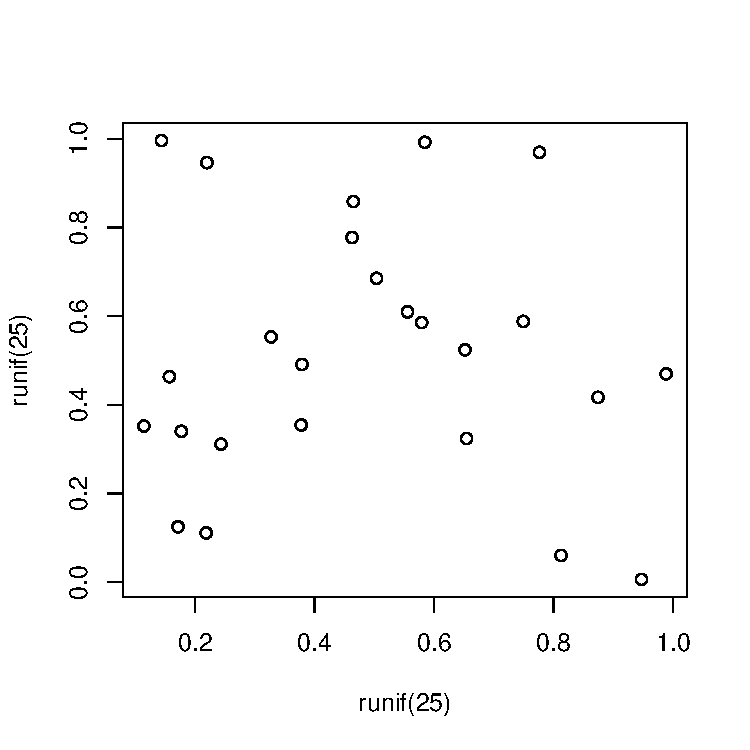
\includegraphics[width=0.5\textwidth,height=\textheight]{Tarea_files/figure-pdf/fig-meaningless-1.pdf}

}

\caption{\label{fig-meaningless}A meaningless scatterplot}

\end{figure}

\hypertarget{tables-coming-from-r}{%
\section{Tables coming from R}\label{tables-coming-from-r}}

Tables can also be generated using R chunks, as shown in
Table~\ref{tbl-simple} example.

\begin{Shaded}
\begin{Highlighting}[]
\NormalTok{knitr}\SpecialCharTok{::}\FunctionTok{kable}\NormalTok{(}\FunctionTok{head}\NormalTok{(mtcars)[,}\DecValTok{1}\SpecialCharTok{:}\DecValTok{4}\NormalTok{])}
\end{Highlighting}
\end{Shaded}

\hypertarget{tbl-simple}{}
\begin{longtable}[]{@{}lrrrr@{}}
\caption{\label{tbl-simple}Caption centered above table}\tabularnewline
\toprule\noalign{}
& mpg & cyl & disp & hp \\
\midrule\noalign{}
\endfirsthead
\toprule\noalign{}
& mpg & cyl & disp & hp \\
\midrule\noalign{}
\endhead
\bottomrule\noalign{}
\endlastfoot
Mazda RX4 & 21.0 & 6 & 160 & 110 \\
Mazda RX4 Wag & 21.0 & 6 & 160 & 110 \\
Datsun 710 & 22.8 & 4 & 108 & 93 \\
Hornet 4 Drive & 21.4 & 6 & 258 & 110 \\
Hornet Sportabout & 18.7 & 8 & 360 & 175 \\
Valiant & 18.1 & 6 & 225 & 105 \\
\end{longtable}


\renewcommand\refname{References}
  \bibliography{bibliography.bib}


\end{document}
